\chapter{Metodologia}

Para se construir um software é necessário seguir uma série de passos previsíveis, esses passos estão definidos no processo de software. Um processo de software pode ser visto como um conjunto de atividades, métodos, práticas e transformações que guiam pessoas na produção de software.

Para a construção do processo há uma adaptação em 3 principais níveis de acordo com o \cite{safe} (portfólio, programa e time):

\begin{itemize}
  \item O nível de portfólio é responsável por gerar boa parte da documentação do projeto aplicando as 3 atividades principais da engenharia de requisitos, que são elicitação, modelagem e análise
  \item O nível de programa é onde irá documentar a arquitetura, as ferramentas de UX e definir o \textit{product backlog} com sua rastreabilidade
  \item O nível de time que é onde irá codificar a solução, está dividido em desenvolvimento que irá executar a sprint e gestão na qual irá aplicar as práticas do scrum, além da infraestrutura e dos testes.
\end{itemize}

Alguns papéis são realizados ao longo do processo, são eles:

\begin{itemize}
  \item \textbf{Scrum Master}: Responsável por garantir que os valores scrum sejam adotados e praticados, ou seja, é o gestor do projeto.
  \item \textbf{Scrum Team}: Transforma o \textit{product backlog} em incrementos de funcionalidades potencialmente entregáveis em cada \textit{Sprint} utilizando de boas práticas definidas no XP.
  \item \textbf{Product Owner}: Responsável por gerenciar o \textit{product backlog} e responsável pelo produto, são os \textit{stakeholders}, ou seja, as pessoas interessadas no software.
  \item \textbf{Devops}: Responsável por toda a parte de infraestrutura e \textit{pipeline} do projeto.
  \item \textbf{Architecture Owner}: Responsável por definir a estrutura, a organização e a forma de manutenção do software.
\end{itemize}

\section{Nível de portfólio: Processo de engenharia de requisitos}

Dentro da Engenharia de Software vários modelos definem as etapas necessárias para se construir um software de acordo com o processo definido, mas todos têm algo em comum: uma etapa dedicada a compreensão dos problemas a serem solucionados e a definição de o quê será feito. Esta etapa inicial recebe o nome de engenharia de requisitos e está localizado no nível de portfólio do SAFe.

O processo definido na figura \ref{fig:requisitos} para a etapa de engenharia de requisitos do software PGTBL segue três atividades principais:

\begin{itemize}
  \item \textbf{Elicitação}: Essa atividade preocupa-se com o levantamento dos principais aspectos, sejam eles funcionais e/ou não funcionais. Podemos dizer que passamos de um alto nível de abstração para algo mais próximo do mundo real utilizando várias técnicas de elicitação, no caso foi utilizado as técnicas de \textit{brainstorm} e prototipagem.
  \item \textbf{Modelagem}: Uma vez elicitados os requisitos, deve-se modelar os mesmo de acordo com uma notação adequada, foi utilizado o framework i* para uma modelagem mais organizacional do projeto, o UML para requisitos funcionais do projeto através do diagrama de classe e o framework NFR para requisitos não funcionais do projeto.
  \item \textbf{Análise}: Essa atividade usa a modelagem para obter maior conhecimento sobre as necessidades do software em investigação, no caso os planos de análise de riscos, custos, tempo, viabilidade técnica e outros aspectos são levados em
consideração.
\end{itemize}

\begin{figure}[h!]
	\centering
  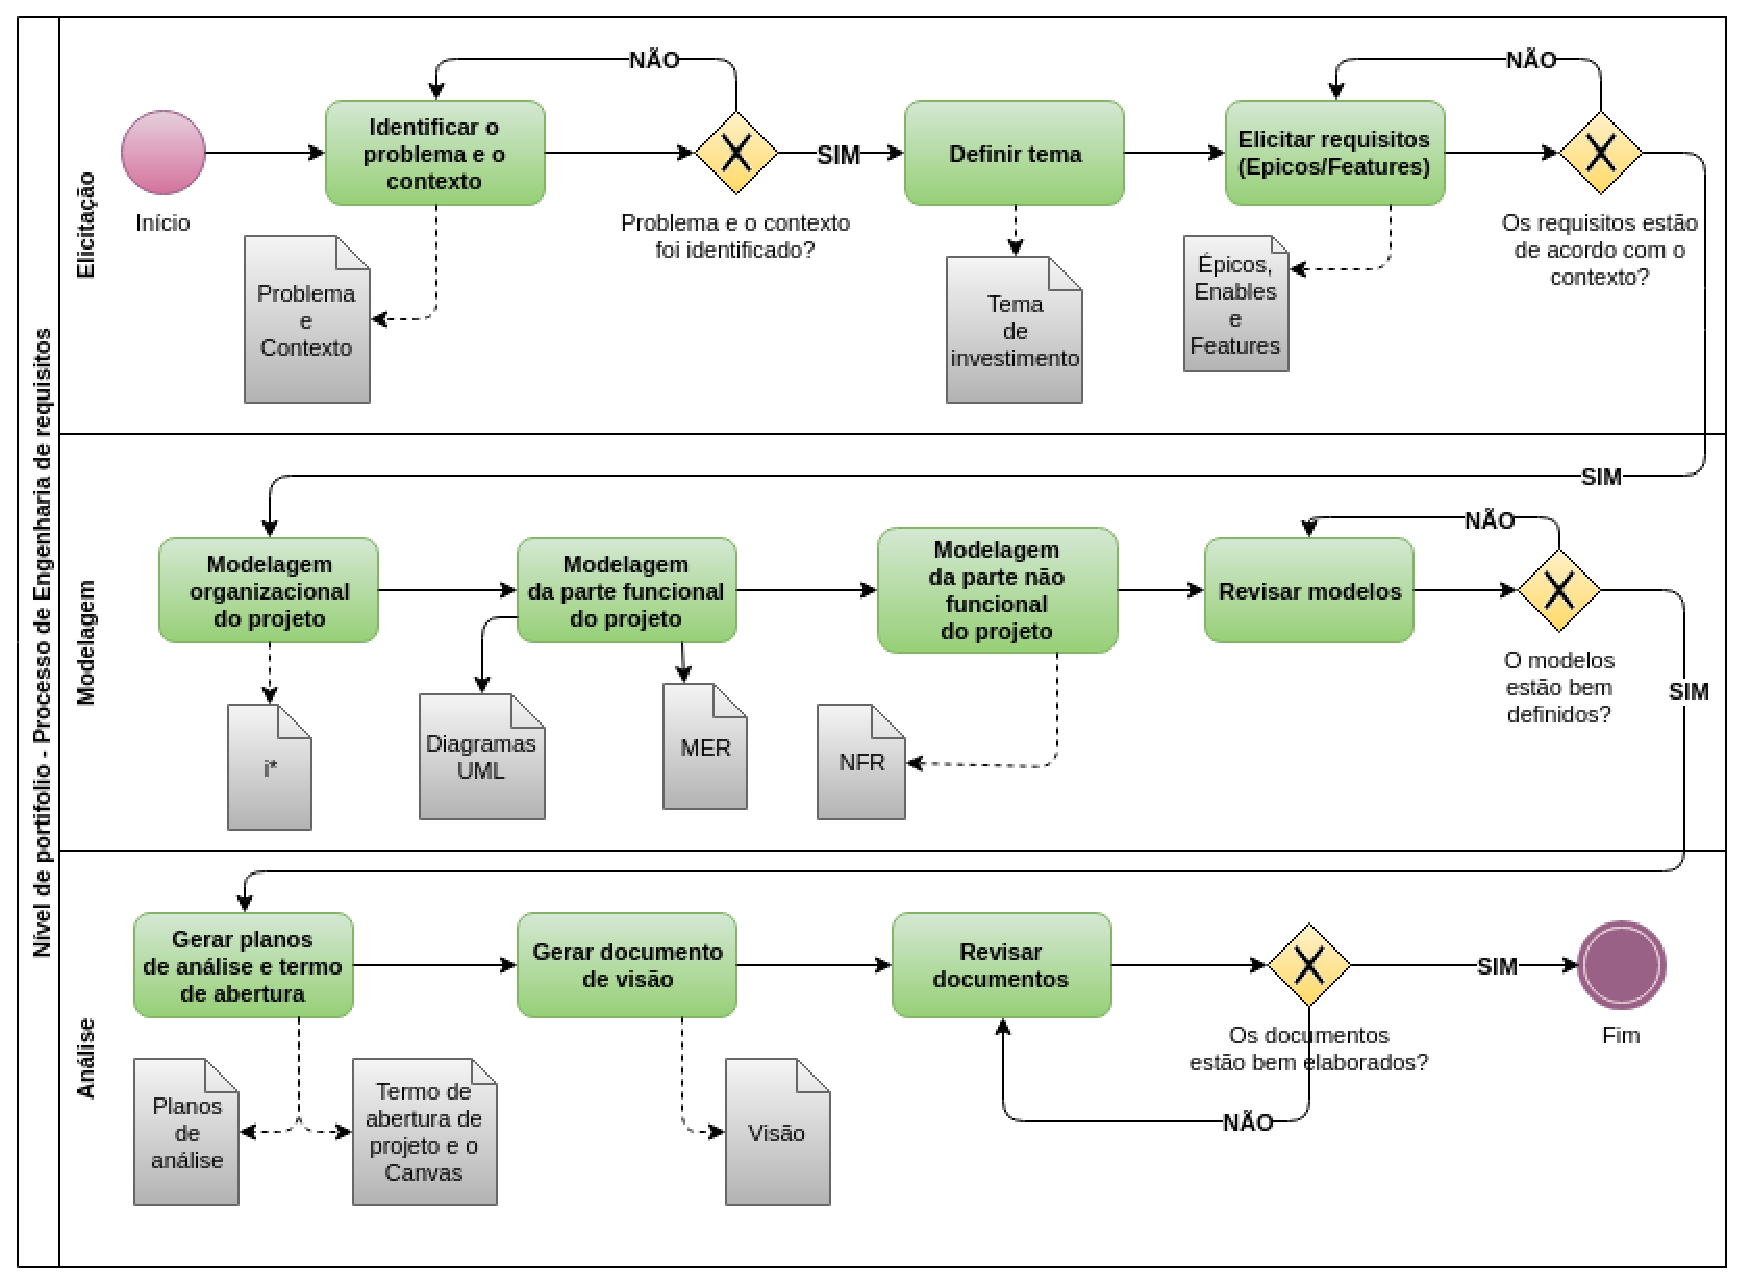
\includegraphics[keepaspectratio=true,scale=0.5]{figuras/requisitos.eps}
  \caption[Processo de engenharia de requisitos.]{Processo de engenharia de requisitos. Fonte: Autor}
	\label{fig:requisitos}
\end{figure}

\subsection{Atividades do processo de engenharia de requisitos (Elicitação)}

\subsubsection{Identificar o problema e o contexto}

\begin{itemize}
  \item \textbf{Descrição}: Nesta etapa, objetiva-se identificar o problema e o contexto na qual o software será aplicado.
  \item \textbf{Responsável}: Scrum Master
  \item \textbf{Envolvidos}: Product Owner
  \item \textbf{Entradas}: N/A
  \item \textbf{Saídas}: Problema e contexto identificado.
\end{itemize}

\subsubsection{Definir tema}

\begin{itemize}
  \item \textbf{Descrição}: Nesta etapa, com o problema e o contexto bem definido será identificado o tema de investimento na qual o software será criado.
  \item \textbf{Responsável}: Scrum Master
  \item \textbf{Envolvidos}: Product Owner
  \item \textbf{Entradas}: Problema e contexto
  \item \textbf{Saídas}: Tema de investimento
\end{itemize}

\subsubsection{Elicitar Requisitos}

\begin{itemize}
  \item \textbf{Descrição}: Nesta etapa, objetiva-se elicitar os requisitos através de técnicas de elicitação como brainstorm e prototipação. É nessa etapa que é identificado os Épicos (requisitos funcionais) e Enables (requisitos não funcionais) por meio do tema de investimento e os Épicos são separado em pedaços menores chamadas Features. Na rastreabilidade os épicos são identificados com a sigla ‘EP’, Enables com a sigla ‘EN’ e as Features com a sigla ‘FE’.
  \item \textbf{Responsável}: Scrum Master e Scrum Team
  \item \textbf{Envolvidos}: Product Owner
  \item \textbf{Entradas}: Tema de investimento
  \item \textbf{Saídas}: Épico, Enables e Features definidos e documentados no documento de \href{https://github.com/VictorArnaud/TBL/wiki/Rastreabilidade-de-requisitos}{Rastreabilidade de requisitos} e \href{https://github.com/VictorArnaud/TBL/wiki/T%C3%A9cnicas-de-elicita%C3%A7%C3%A3o}{Técnicas de elicitação}.
\end{itemize}

\subsection{Atividades do processo de engenharia de requisitos (Modelagem)}

\subsubsection{Modelagem organizacional do projeto}

\begin{itemize}
  \item \textbf{Descrição}: Nesta etapa, objetiva-se criar um modelo organizacional em contexto com o uso do software.  Essa modelagem foi feito utilizando um framework chamado i* (i-estrela) originalmente proposto por Yu, trata da modelagem de contextos organizacionais tomando como base os relacionamentos de dependência entre os atores participantes. É dividido em Modelo SD (modelo de dependência estratégicas externa) e modelo SR (modelo de dependência estratégica interna)
  \item \textbf{Responsável}: Architecture Owner e Scrum Team
  \item \textbf{Envolvidos}: N/A
  \item \textbf{Entradas}: Features
  \item \textbf{Saídas}: \href{https://victorarnaud.github.io/TBL/contribuicao/arquitetura/#4-framework-i}{i* modelo SR e SD} no documento de arquitetura do software.
\end{itemize}

\subsubsection{Modelagem da parte funcional do projeto}

\begin{itemize}
  \item \textbf{Descrição}: Nesta etapa, objetiva-se criar diagramas que auxilia na construção das funcionalidades do software por meio da modelagem UML como Diagrama de classe e criar a modelagem do banco de dados relacional por meio do Modelo Entidade Relacionamento (MER).
  \item \textbf{Responsável}: Architecture Owner e Scrum Team
  \item \textbf{Envolvidos}: N/A
  \item \textbf{Entradas}: Features
  \item \textbf{Saídas}: \href{https://victorarnaud.github.io/TBL/contribuicao/arquitetura/#3-diagrama-de-classe}{Diagrama de classe} e \href{https://victorarnaud.github.io/TBL/contribuicao/arquitetura/#3-diagrama-de-classe}{MER} no documento de arquitetura do software.
\end{itemize}

\subsubsection{Modelagem da parte não funcional do projeto}

\begin{itemize}
  \item \textbf{Descrição}: Nesta etapa, objetiva-se criar diagramas que auxilia a identificar requisitos não funcionais do software como metas a serem alcançadas por meio do framework NFR.
  \item \textbf{Responsável}: Architecture Owner e Scrum Team
  \item \textbf{Envolvidos}: N/A
  \item \textbf{Entradas}: Enables
  \item \textbf{Saídas}: \href{https://victorarnaud.github.io/TBL/contribuicao/arquitetura/#5-framework-nfr}{Framework NFR} no documento de arquitetura do software.
\end{itemize}

\subsubsection{Revisar modelos}

\begin{itemize}
  \item \textbf{Descrição}: Nesta etapa, objetiva-se revisar todos os diagramas em cada iteração do ciclo de desenvolvimento.
  \item \textbf{Responsável}: Architecture Owner e Scrum Master
  \item \textbf{Envolvidos}: Product Owner
  \item \textbf{Entradas}: i*, NFR, MER e Diagrama de Classe
  \item \textbf{Saídas}: i*, NFR, MER e Diagrama de classe refinados
\end{itemize}

\subsection{Atividades do processo de engenharia de requisitos (Análise)}

\subsubsection{Gerar planos de análise}

\begin{itemize}
  \item \textbf{Descrição}: Nesta etapa, objetiva-se criar todos os documentos relacionados ao gerenciamento do projeto, como por exemplo, documento de abertura do projeto, que terá um resumo dos documentos de gerenciamento como plano de gerenciamento de recursos humanos, comunicação, risco, medição e análise, configuração de software, aquisição e custos.
  \item \textbf{Responsável}: Scrum Master
  \item \textbf{Envolvidos}: N/A
  \item \textbf{Entradas}: Modelo organizacional, funcional e não funcional
  \item \textbf{Saídas}: \href{https://github.com/VictorArnaud/TBL/wiki/Planos-de-gerenciamento}{Planos de análise}, \href{https://victorarnaud.github.io/TBL/tap/}{Termo de abertura de projeto}, \href{https://victorarnaud.github.io/TBL/canvas/}{Canvas}.
\end{itemize}

\subsubsection{Gerar documento de visão}

\begin{itemize}
  \item \textbf{Descrição}: Nesta etapa, objetiva-se criar o documento de visão do produto
  \item \textbf{Responsável}: Scrum Master e Scrum Team
  \item \textbf{Envolvidos}: Product Owner
  \item \textbf{Entradas}: Requisitos, Planos de análise, Termo de abertura e Canvas
  \item \textbf{Saídas}: \href{https://victorarnaud.github.io/TBL/visao/}{Documento de visão}
\end{itemize}

\subsubsection{Revisar documentos}

\begin{itemize}
  \item \textbf{Descrição}: Nesta etapa, objetiva-se revisar os documentos criados anteriormente
  \item \textbf{Responsável}: Scrum Master e Scrum Team
  \item \textbf{Envolvidos}: Product Owner
  \item \textbf{Entradas}: Documento de visão, Planos de análise, Termo de abertura e Canvas
  \item \textbf{Saídas}: Documentos revisados e refinados
\end{itemize}

\section{Nível de programa e Time: Processo de desenvolvimento}

A construção do software foi feito seguindo uma adaptação das metodologias ágeis SCRUM, XP e SAFe para aumentar a produtividade e eficiência do mesmo, já que o projeto todo foi feito por uma única pessoa, ou seja, teve toda uma adaptação para isso.

Foi seguido o SCRUM e XP para o gerenciamento e desenvolvimento projeto respectivamente e o SAFe para a rastreabilidade dos requisitos.

O gerenciamento da sprint foi feito por quadros Kanban, na qual teremos nove quadros principais. Esses quadros se encontram nos Boards do github, utilizando como base o plugin chamado \href{https://www.zenhub.com/}{Zenhub}. Para instalar é só baixar o plugin e instalar no navegador, a partir daí já conseguirá ver toda organização das issues do projeto a partir da ferramenta. Os quadros são:

\begin{itemize}
  \item \textbf{Epic}: Épicos do software.
  \item \textbf{Features}: \textit{Features} do software.
  \item \textbf{New issues}: Novas histórias de usuário, bug reports ou qualquer tipo de situações de trabalho relacionadas ao desenvolvimento da aplicação que ainda não foram mapeadas, pontuadas ou priorizadas e consequentemente alocadas nos demais quadros.
  \item \textbf{Ice Box}: Issues congeladas por dependência de outras, por alguma necessidade de reavaliação da necessidade ou do esforço necessário para concluí-la, por dependência de funcionalidades externas que não são disponibilizadas pelos mantenedores, por temporária incapacidade da equipe de solucionar determinado problema, etc.
  \item \textbf{Product Backlog}: \textit{Board} para histórias/tarefas ou correções já mapeadas e priorizadas. É importante esclarecer que nesse quadro, a prioridade é definida pela posição da \textit{issue} na \textit{board}, sendo que as posições superiores determinam maior relevância para o projeto.
  \item \textbf{Sprint Backlog}: \textit{Issues} alocadas para os pares na \textit{sprint} corrente ou \textit{bug fixes} de alta prioridade.
  \item \textbf{Review}: Tarefas concluídas que necessitam de revisão para entrarem na aplicação.
  \item \textbf{Done}: Código já revisado que pode ser anexado a aplicação na próxima release.
  \item \textbf{Closed}: \textit{Issues} fechadas já anexado a aplicação.
\end{itemize}

Na figura \ref{fig:desenvolvimento} está definido o processo de desenvolvimento que está no nível de programa e time.

\begin{figure}[h!]
	\centering
  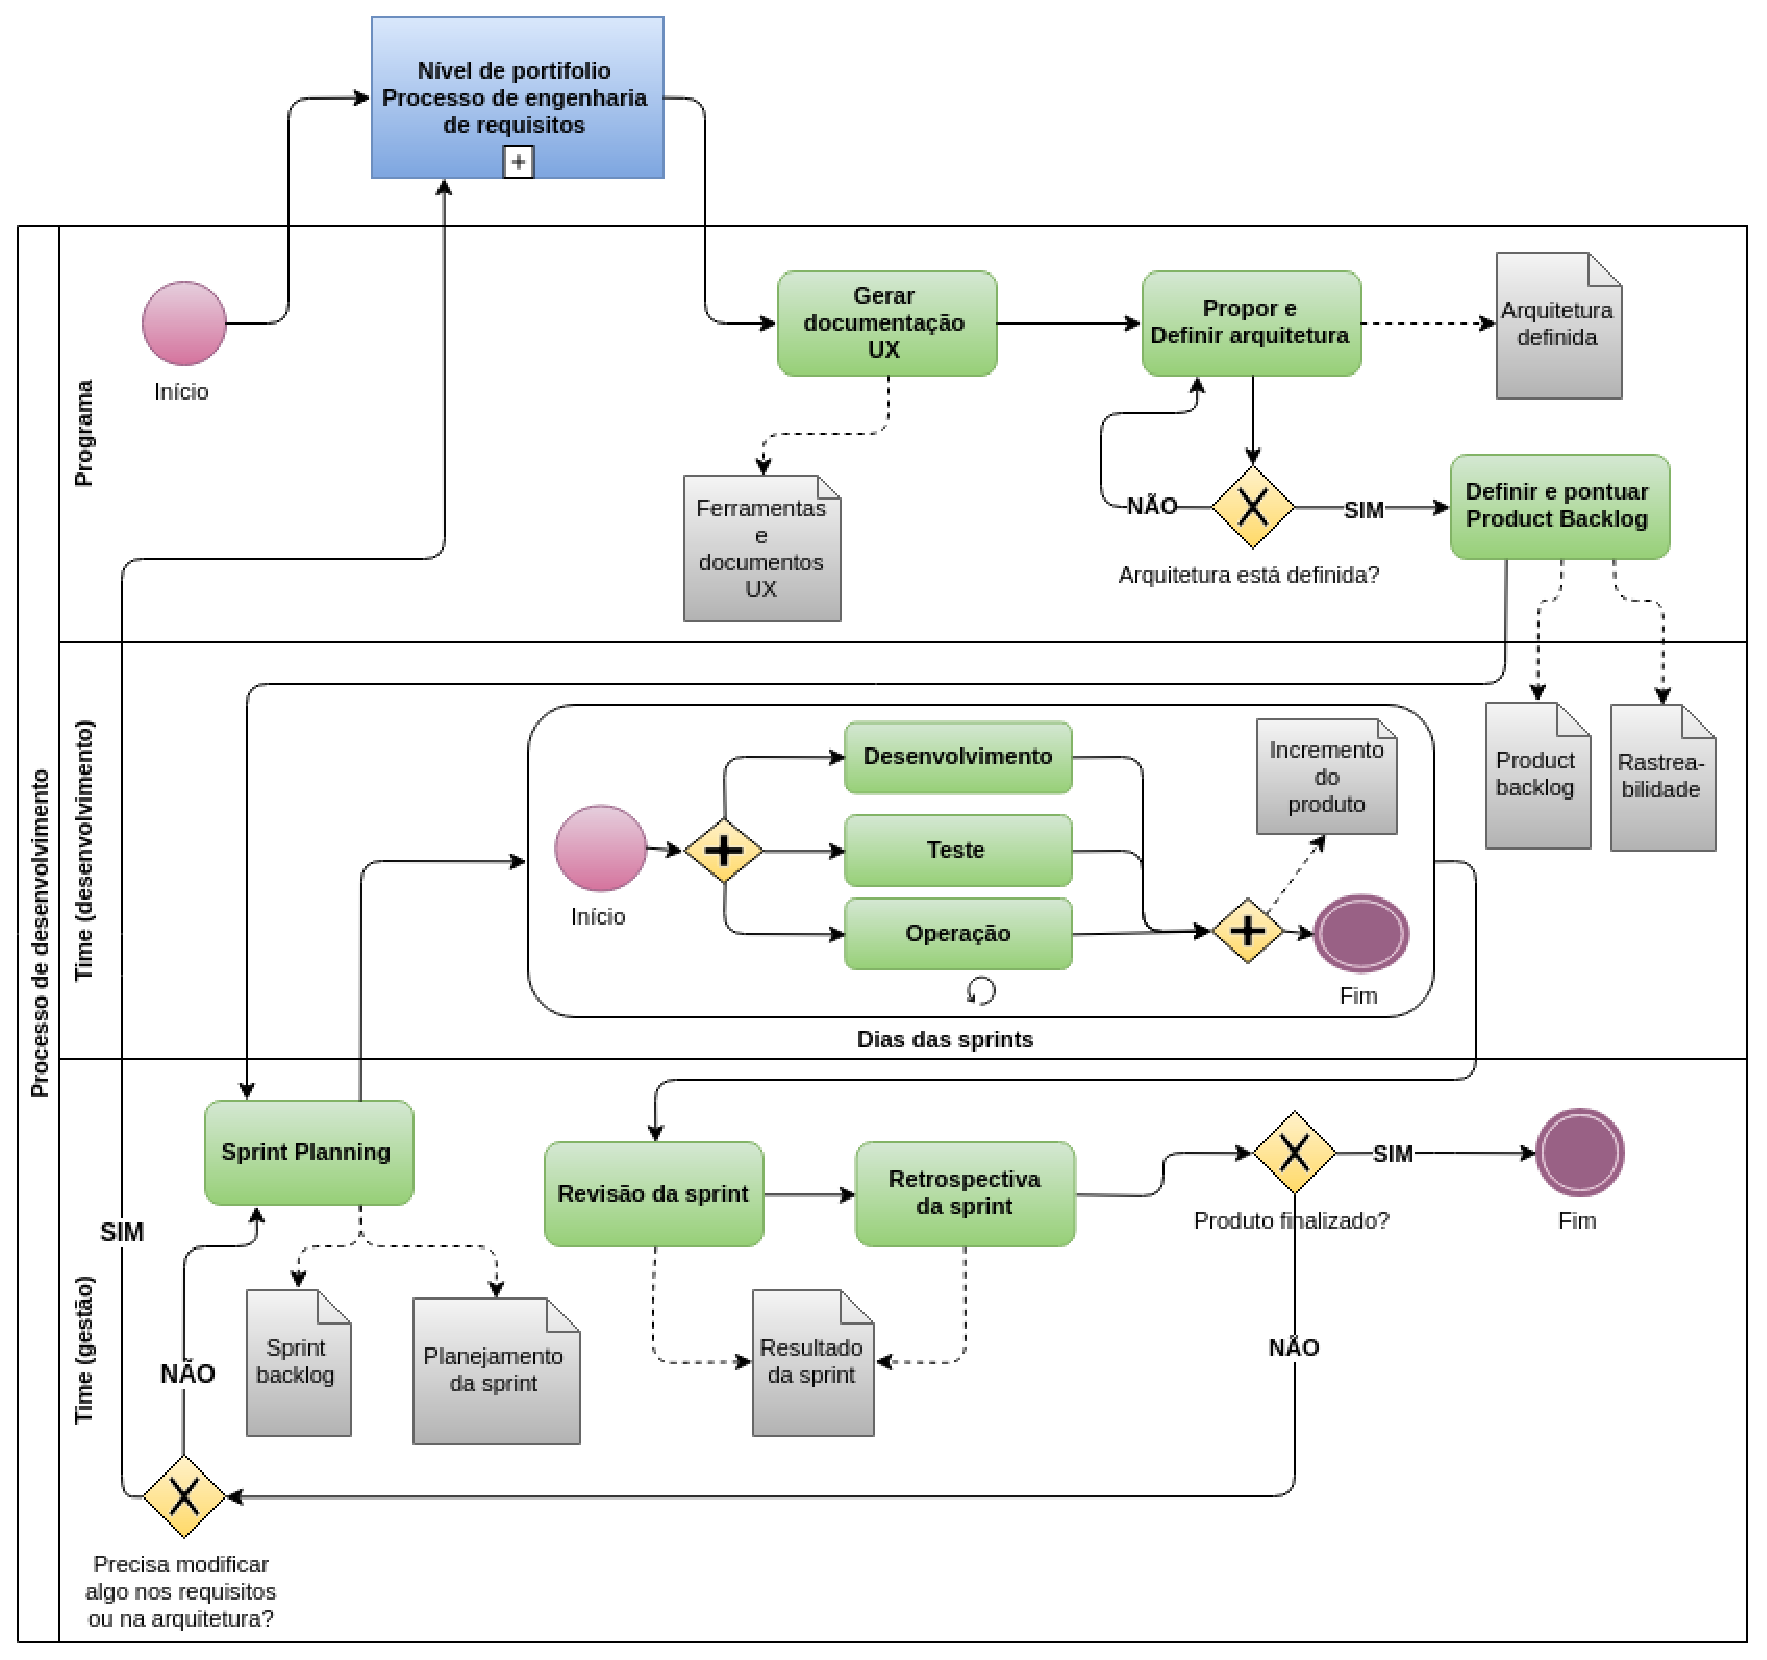
\includegraphics[keepaspectratio=true,scale=0.5]{figuras/desenvolvimento.eps}
  \caption[Processo de desenvolvimento.]{Processo de desenvolvimento. Fonte: Autor}
	\label{fig:desenvolvimento}
\end{figure}

Todo processo definido será executado de forma incremental por iterações, ou seja, a cada iteração será realizada um
refinamento dos documentos e um incremento do produto, essas iterações são chamadas \textit{Sprints}.

\subsection{Nível de programa}

Fase responsável pela auto-organização de times ágeis, entrega contínua de valor, criação de Features por meio dos épicos encontrados, realização de toda a documentação relacionada ao \textit{User Experience} ou UX, e definição do documento de arquitetura do software.

\subsubsection{Gerar documentação UX}

\begin{itemize}
  \item \textbf{Descrição}: Nesta etapa, objetiva-se criar os documentos UX relevantes para o projeto como protótipos, sitemaps, entre outros.
  \item \textbf{Responsável}: Architecture Owner
  \item \textbf{Envolvidos}: N/A
  \item \textbf{Entradas}: Requisitos e modelos
  \item \textbf{Saídas}: Ferramentas e documentos UX como \href{https://victorarnaud.github.io/TBL/sitemap/}{sitemap}, \href{https://victorarnaud.github.io/TBL/storyboards/}{StoryBoards} e \href{https://github.com/VictorArnaud/TBL/wiki/Prot%C3%B3tipo}{Prototipo}
\end{itemize}

\subsubsection{Propor e definir arquitetura}

\begin{itemize}
  \item \textbf{Descrição}: Nesta etapa, objetiva-se propor e definir a arquitetura que melhor se adapte ao projeto e a equipe.
  \item \textbf{Responsável}: Architecture Owner, Scrum Team e Devops
  \item \textbf{Envolvidos}: N/A
  \item \textbf{Entradas}: Requisitos e modelos
  \item \textbf{Saídas}: \href{https://victorarnaud.github.io/TBL/contribuicao/arquitetura/}{Documento de arquitetura}
\end{itemize}

\subsubsection{Definir e pontuar product backlog}

\begin{itemize}
  \item \textbf{Descrição}: Nesta etapa, objetiva-se definir e pontuar as histórias de usuário do product backlog para a release que segue.
  \item \textbf{Responsável}: Scrum Master, Scrum Team e Devop
  \item \textbf{Envolvidos}: Product Owner
  \item \textbf{Entradas}: Features e Enables
  \item \textbf{Saídas}: \href{https://github.com/VictorArnaud/TBL/wiki/Product-Backlog}{Product Backlog} e \href{https://github.com/VictorArnaud/TBL/wiki/Rastreabilidade-de-requisitos}{Rastreabilidade}.
\end{itemize}

\subsection{Nível de time (Gestão e Desenvolvimento)}

Fase responsável pelo auto-gerenciamento da equipe ágil, incremento do software totalmente testado, práticas SCRUM e XP, descrição do valor por meio de User Stories e tarefas.

\subsubsection{Sprint Planning}

\begin{itemize}
  \item \textbf{Descrição}: Nesta etapa, objetiva-se priorizar as histórias de usuários que serão implementadas na
    iteração/sprint que se segue. Os planejamentos e Resultados encontram-se na wiki do projeto.
  \item \textbf{Responsável}: Scrum Master, Scrum Team e Devops
  \item \textbf{Envolvidos}: N/A
  \item \textbf{Entradas}: Product Backlog
  \item \textbf{Saídas}: Sprint Backlog e Planejamento das sprints
\end{itemize}

\subsubsection{Ciclo de dias das sprints}

\begin{itemize}
  \item \textbf{Descrição}: Nesta etapa, será aplicado às boas práticas do SCRUM e XP em nível de desenvolvimento. Foram retirados algumas atividades do SCRUM como Daily Scrum, e práticas XP como programação pareada, já que a equipe é composta de um único membro, não há como fazer. Dentro dessa atividade temos em paralelo o desenvolvimento, teste e operações do incremento do produto.
  \item \textbf{Responsável}: Scrum Team e Devops
  \item \textbf{Envolvidos}: N/A
  \item \textbf{Entradas}: Sprint Backlog
  \item \textbf{Saídas}: Incremento do produto testado e em homologação
\end{itemize}

\subsubsection{Revisão da sprint}

\begin{itemize}
  \item \textbf{Descrição}: Nesta etapa, será apresentado as funcionalidades implementadas na sprint e verificar se há alguma dívida técnica para a próxima sprint que se segue.
  \item \textbf{Responsável}: Scrum Master, Scrum Team e Devops
  \item \textbf{Envolvidos}: Product Owner
  \item \textbf{Entradas}: Incremento do produto
  \item \textbf{Saídas}: Resultados da sprin
\end{itemize}

\subsubsection{Retrospectiva da sprint}

\begin{itemize}
  \item \textbf{Descrição}: Nesta etapa, será coletado pontos positivos, negativos e melhorias para as próximas iterações da equipe
  \item \textbf{Responsável}: Scrum Master, Scrum Team e Devops
  \item \textbf{Envolvidos}: Product Owner
  \item \textbf{Entradas}: Pontos positivos, negativos e melhorias
  \item \textbf{Saídas}: Resultados da sprint
\end{itemize}
